% !TeX program = xelatex
% !TeX encoding = UTF-8
% !TeX TXS-program:compile = txs:///xelatex | txs:///xelatex
\documentclass[aspectratio=169, table, 12pt]{beamer}

% Preamble bersama seluruh slide mata kuliah ini.
% Dipanggil dari slides/sessionXX/sessionXX.tex tepat sesudah baris
% \documentclass[aspectratio=169, table, 12pt]{beamer}
% Paket tambahan yang hanya dibutuhkan satu sesi ditulis di berkas sesi itu.

\usepackage{colortbl}
\usepackage{xcolor}
\usepackage{listings}
\usepackage{tabularx}
\usepackage{booktabs}
\usepackage{tikz}
\usepackage{pgfplots}
\usepackage{fontspec}
\usepackage[english,bahasai]{babel}
\pgfplotsset{compat=1.18}
\usetikzlibrary{arrows.meta, positioning, calc, fit, shapes.geometric,
  shapes.multipart, backgrounds, matrix, chains, trees}

\makeatletter
\def\input@path{{../theme/}}
\makeatother
\graphicspath{{../theme/}{../../figures/}}
% Stub symlink Windows memakai tema cadangan sampai aset institusi tersedia.
\IfFileExists{../theme/beamerthemePradita.sty}{%
  \usetheme{Pradita}
}{%
  \usetheme{Madrid}
  \setmainfont{TeX Gyre Heros}
  \setsansfont{TeX Gyre Heros}
  \setbeamertemplate{navigation symbols}{}
}

\definecolor{praditagreen}{RGB}{37, 113, 71}
\setbeamercolor{structure}{fg=praditagreen}
\setbeamercolor{palette primary}{bg=praditagreen,fg=white}
\setbeamercolor{palette secondary}{bg=praditagreen!80!black,fg=white}
\setbeamercolor{palette tertiary}{bg=praditagreen!60!black,fg=white}
\setbeamerfont{frametitle}{size=\large}
\setbeamertemplate{caption}[numbered]

% Ukuran header mengikuti teks agar judul panjang tidak menabrak logo.
\setbeamercolor{frametitle}{bg=white,fg=black}
\setbeamertemplate{frametitle}{%
  \begin{beamercolorbox}[wd=\paperwidth,sep=0.2cm]{frametitle}
    \begin{minipage}[c]{0.77\paperwidth}
      \raggedright\fontsize{16}{18}\selectfont\bfseries\insertframetitle
      \ifx\insertframesubtitle\empty\else
        \par\small\mdseries\insertframesubtitle
      \fi
    \end{minipage}\hfill
    \begin{minipage}[c]{0.15\paperwidth}
      \IfFileExists{../theme/classFiles/logo_universitas.png}{%
        
\includegraphics[width=\linewidth]{../theme/classFiles/logo_universitas.png}%
      }{}
    \end{minipage}
  \end{beamercolorbox}
}
\setbeamertemplate{footline}{%
  \ifnum\value{framenumber}>1
    \begin{beamercolorbox}[wd=\paperwidth,ht=0.35cm,dp=0.15cm,
      leftskip=0.3cm,rightskip=0.3cm]{palette primary}
      \footnotesize\bfseries\insertframenumber/\inserttotalframenumber
      \hfill IT40813
    \end{beamercolorbox}
  \fi
}
\DeclareRobustCommand{\berkas}[1]{\path{#1}}

% Tema membuat garis tabel berwarna putih. Dikembalikan agar tabel terbaca.
\arrayrulecolor{black}
\setlength{\arrayrulewidth}{0.5pt}

\lstdefinelanguage{yaml}{
  basicstyle=\ttfamily\scriptsize,
  keywordstyle=\color{blue}\bfseries,
  commentstyle=\color{gray}\itshape,
  stringstyle=\color{red},
  showstringspaces=false,
  breaklines=true,
  frame=lines,
  numbers=none,
  backgroundcolor=\color{lightgray!10},
  tabsize=2,
  morecomment=[l]{\#}
}

\lstdefinelanguage{json}{
  basicstyle=\ttfamily\scriptsize,
  stringstyle=\color{red},
  commentstyle=\color{gray},
  breaklines=true,
  showstringspaces=false,
  tabsize=2,
  numbers=none,
  frame=lines,
  backgroundcolor=\color{lightgray!10},
  string=[s]{"}{"}
}

\lstdefinelanguage{bash}{
  keywords={},
  basicstyle=\ttfamily\scriptsize,
  ndkeywords={docker, kubectl, helm, curl, git, terraform},
  ndkeywordstyle=\color{purple}\bfseries,
  sensitive=true,
  commentstyle=\color{gray},
  numbers=none,
  breaklines=true,
  frame=lines,
  backgroundcolor=\color{lightgray!10},
  tabsize=2,
  comment=[l]{\#},
  showstringspaces=false
}

\lstdefinelanguage{http}{
  keywords={GET, POST, PUT, PATCH, DELETE, HEAD, OPTIONS, HTTP},
  basicstyle=\ttfamily\scriptsize,
  keywordstyle=\color{blue}\bfseries,
  sensitive=true,
  numbers=none,
  breaklines=true,
  frame=lines,
  backgroundcolor=\color{lightgray!10},
  tabsize=2,
  showstringspaces=false
}

\subtitle{IT40813 · IT Governance, Risk \& Compliance}
\author{\textbf{Alfa Yohannis}}


% Sampul membatasi judul di panel putih tema rujukan Pradita.
\setbeamertemplate{title page}{%
  \begin{tikzpicture}[remember picture,overlay]
    \node[anchor=north west,inner sep=0pt,text width=8.8cm]
      at ([xshift=1cm,yshift=-3.15cm]current page.north west) {%
        {\small\insertsubtitle\par}\vspace{0.25cm}
        \resizebox{8.8cm}{!}{\begin{minipage}{12cm}
          \raggedright\color{praditagreen}\bfseries\inserttitle
        \end{minipage}}
      };
    \node[anchor=south west,inner sep=0pt]
      at ([xshift=1cm,yshift=1.65cm]current page.south west)
      {\small\insertdate};
    \node[anchor=west,inner sep=0pt,text=white]
      at ([xshift=0.8cm,yshift=0.75cm]current page.south west)
      {\small\insertauthor};
  \end{tikzpicture}
}


\title{\Huge Orientasi Mata Kuliah\\ \vspace{10pt} dan Dasar-Dasar GRC}
\date{Pertemuan 01}

\begin{document}

\frame{\titlepage}

\begin{frame}
  \frametitle{Isi Pertemuan}
  \vspace{14pt}
  \begin{columns}[t]
    \column{0.5\textwidth}
    {\small\tableofcontents[sections={1-3}]}

    \column{0.5\textwidth}
    {\small\tableofcontents[sections={4-6}]}
  \end{columns}
\end{frame}

\begin{frame}{\hfill}
  \centering
  \Huge{\textbf{Setelah data pasien bocor\\lewat vendor, siapa yang\\berhak memutuskan\\perbaikannya?}}
\end{frame}

\section{Tujuan dan Konteks}

\begin{frame}{\hfill}
  \centering
  \Huge{\textbf{Tujuan dan Konteks}}
\end{frame}

\begin{frame}{{\Large Tujuan Pembelajaran}}
  \vspace{10pt}
  \begin{itemize}
    \item Membedakan tata kelola, manajemen, risiko, kontrol, kepatuhan, dan asurans
          dengan contoh dari organisasi tempat bekerja.
    \item Menjelaskan peran mata kuliah ini dalam capstone bersama dan luaran yang
          disumbangkan ke tiap tonggak.
    \item Memetakan pemangku kepentingan dan pemicu GRC pada organisasi yang dipilih tim.
  \end{itemize}
\end{frame}

\begin{frame}{{\Large Masalah: Tiga Jawaban, Satu Pertanyaan}}
  \vspace{6pt}
  \small
  \begin{itemize}
    \item Unit teknologi menunjuk konfigurasi, pengadaan menunjuk kontrak, dan vendor menunjuk
          instruksi pelanggan.
    \item Ketiganya mungkin benar, tetapi pemutus perbaikan dan pemeriksa hasilnya belum jelas.
    \item Medikara Health menghadapi keadaan ini setelah kebocoran data lewat vendor pada 2025.
    \item Analisis dimulai dari layanan pasien, bukan dari daftar produk keamanan.
    \item Luaran sesi ini masuk tonggak C1 capstone.
  \end{itemize}
\end{frame}

\begin{frame}{{\Large Diagram Konsep Bab 1}}
  \centering
  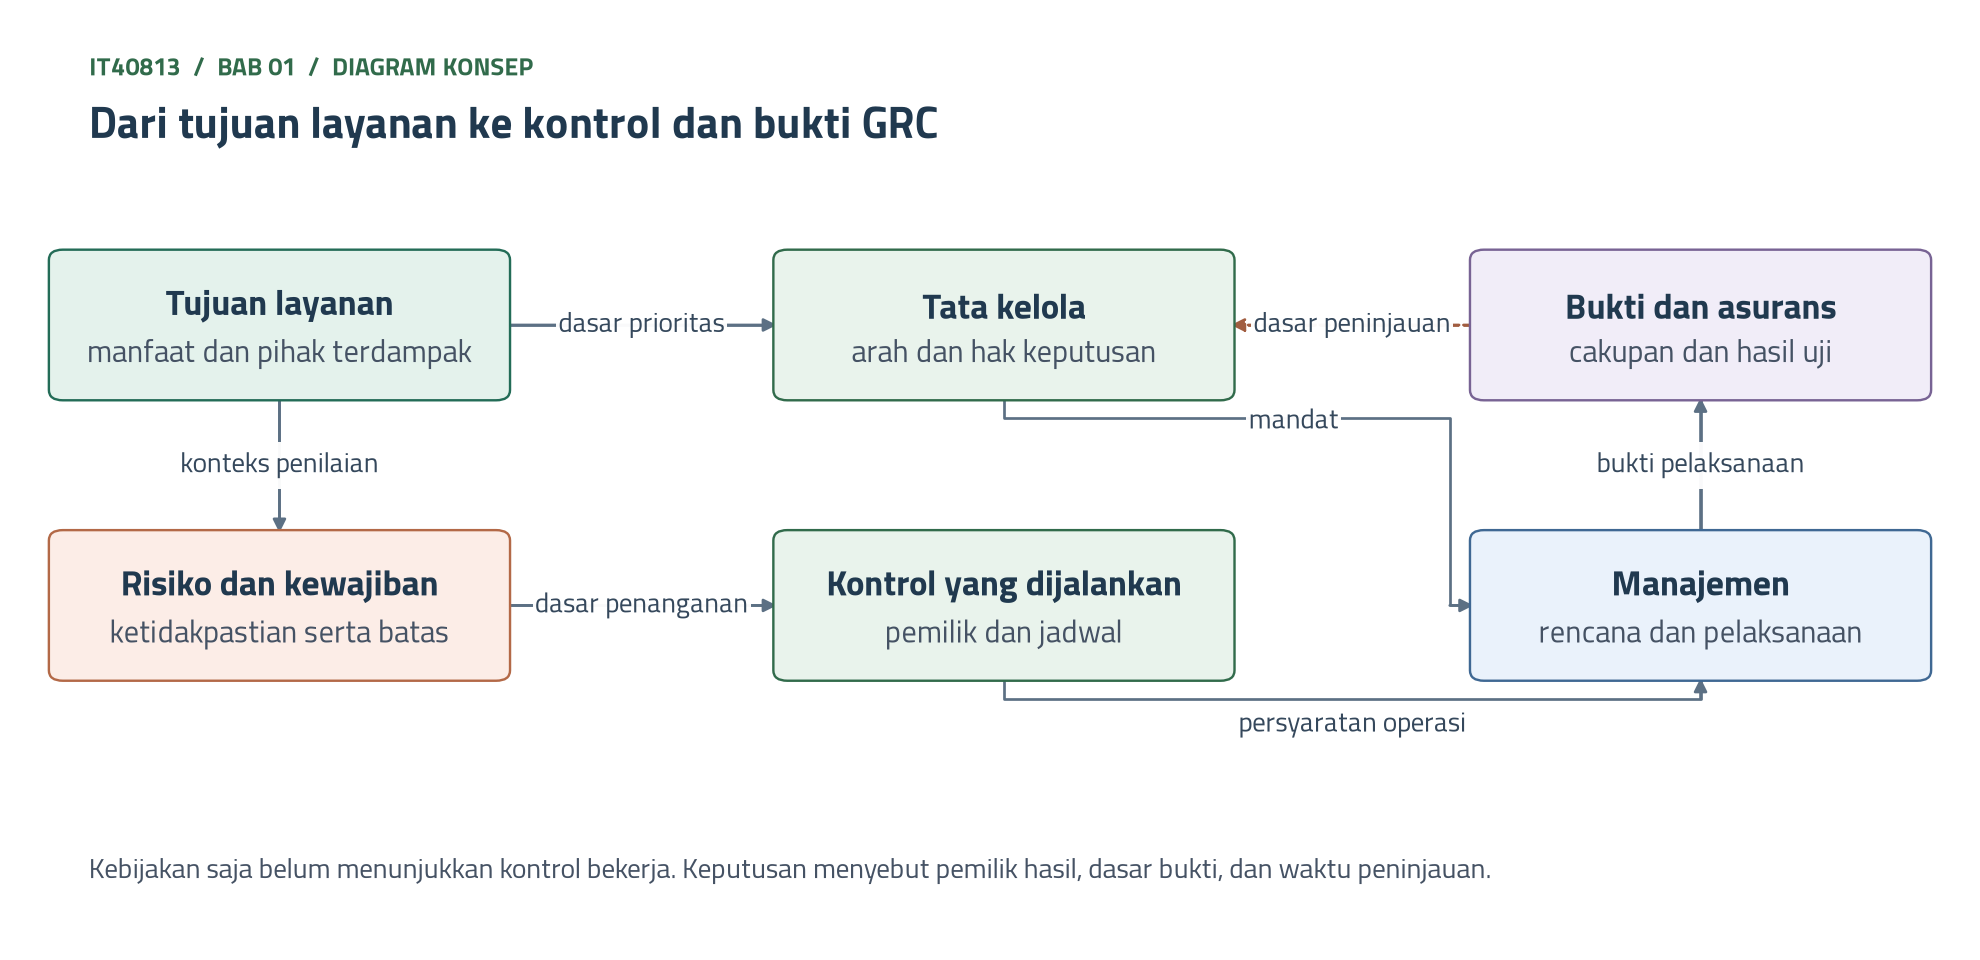
\includegraphics[width=0.96\textwidth,height=0.77\textheight,keepaspectratio]{../../figures/ch01-diagram-konsep.png}
  \label{fig:session01-ilustrasi-bab}
\end{frame}

\section{Mengapa Tata Kelola TI}

\begin{frame}{\hfill}
  \centering
  \Huge{\textbf{Mengapa Organisasi\\Membutuhkan Tata Kelola TI}}
\end{frame}

\begin{frame}{{\Large Tata Kelola TI}}
  \vspace{4pt}
  \small
  \begin{itemize}
    \item Menetapkan arah, hak keputusan, dan cara meminta pertanggungjawaban.
    \item Weill dan Ross: menghubungkan keputusan TI dengan tujuan perusahaan, sekaligus
          memantau kinerja dan akuntabilitas.
    \item Masalah teknis menjadi masalah tata kelola bila menyentuh manfaat, risiko, sumber
          daya, atau hak pihak lain.
    \item Keputusan yang baik menyebut masalah, alternatif, pihak terdampak, dasar, dan waktu
          peninjauan.
  \end{itemize}
  \vspace{4pt}
  {\footnotesize Analogi: pengelola gedung tidak cukup membeli alarm. Pengelola menetapkan siapa
  memeriksa alarm, siapa memimpin evakuasi, dan bagaimana penghuni tahu jalur keluar.}
\end{frame}

\begin{frame}{{\Large Dua Contoh dari Medikara}}
  \vspace{6pt}
  \small
  \begin{itemize}
    \item Misalkan antrean pendaftaran pada 18 klinik turun dari 40 menjadi 25 menit.
    \item Direktur pelayanan memiliki hasil, kepala TI memegang kesiapan sistem.
    \item Misalkan integrasi baru untuk Medikara+ menelan Rp450 juta per tahun.
    \item 28.000 janji temu per bulan berarti 336.000 per tahun, atau sekitar Rp1.340 per janji temu.
    \item Pembandingnya nilai layanan dan biaya integrasi lama, bukan hanya harga implementasi.
  \end{itemize}
\end{frame}

\begin{frame}{{\Large Tiga Gejala Kekosongan Tata Kelola}}
  \vspace{4pt}
  \small
  \begin{itemize}
    \item Proyek gagal: dari 1.471 proyek TI, pembengkakan rata-rata 27 persen, tetapi satu dari
          enam rata-rata 200 persen.
    \item Misalkan anggaran Rp10 miliar: menjadi Rp12,7 miliar, atau Rp30 miliar pada kelompok ekstrem.
    \item Data bocor: pihak ketiga terlibat pada 48 persen pelanggaran, naik dari 30 persen
          (Verizon 2026).
    \item Temuan audit: misalkan 6 dari 30 akun vendor belum dicabut, atau 20 persen sampel.
    \item Angka global memandu pertanyaan, bukan meramal kerugian satu organisasi.
  \end{itemize}
\end{frame}

\begin{frame}{{\Large Pemicu GRC Medikara}}
  \vspace{4pt}
  \footnotesize
  \begin{tabularx}{\textwidth}{|>{\raggedright\arraybackslash}p{0.27\textwidth}|>{\raggedright\arraybackslash}X|>{\raggedright\arraybackslash}X|}
    \hline
    \textbf{Pemicu} & \textbf{Pertanyaan organisasi} & \textbf{Bukti awal} \\ \hline
    Kebocoran vendor 2025 & Siapa membatasi akses vendor? & Kontrak dan daftar akun \\ \hline
    Temuan kontrol akses & Siapa menutup temuan dan kapan? & Laporan audit \\ \hline
    Antrean panjang & Siapa memiliki hasil layanan? & Waktu tunggu agregat \\ \hline
    Biaya integrasi tinggi & Integrasi mana yang memberi nilai? & Biaya dan manfaat \\ \hline
  \end{tabularx}

  \vspace{8pt}
  \small Keempat pemicu adalah fakta dasar kasus. Besarnya masih perlu diukur.
\end{frame}

\begin{frame}{{\Large Kasus Medikara: Insiden Vendor 2025}}
  \vspace{4pt}
  \small
  \begin{itemize}
    \item Fakta dasar: kebocoran data pasien skala kecil lewat vendor pada 2025.
    \item Data latihan: kontrak selesai, tetapi akun dukungan vendor tetap aktif.
    \item 8 malam, 155 panggilan per malam, 1.240 rekam kunjungan. Diketahui pada hari ke-11
          lewat keluhan pasien.
    \item 1.240 rekam setara sekitar 0,1 persen kunjungan setahun. Biaya langsung Rp23,7 juta.
    \item Pertanyaan tetap: siapa mencabut akun, siapa memantau, siapa memutuskan pemberitahuan?
  \end{itemize}
\end{frame}

\section{Tata Kelola dan Istilah Dasar}

\begin{frame}{\hfill}
  \centering
  \Huge{\textbf{Tata Kelola, Manajemen,\\dan Istilah Dasar}}
\end{frame}

\begin{frame}{{\Large Tata Kelola dan Manajemen}}
  \vspace{4pt}
  \small
  \begin{itemize}
    \item Tata kelola: menilai pilihan, memberi arah, dan memantau hasil.
    \item Manajemen: merencanakan, membangun, menjalankan, dan memantau sesuai arah.
    \item COBIT 2019: 40 objektif dalam lima domain, satu tata kelola dan empat manajemen.
    \item ISO/IEC 38500:2024 memakai tiga tugas yang sama untuk badan pengarah.
  \end{itemize}
  \vspace{6pt}
  {\footnotesize Analogi: pemilik restoran menentukan jenis layanan, batas harga, dan standar
  kebersihan. Manajer dapur menyusun giliran kerja dan memeriksa bahan.}
\end{frame}

\begin{frame}{{\Large Pembagian Tugas dan Arus Informasi}}
  \centering
  \resizebox{!}{0.74\textheight}{\begin{tikzpicture}[
  pita/.style={draw,rounded corners,fill=praditagreen!15,minimum width=11.4cm,
    minimum height=1.95cm},
  pita2/.style={pita,fill=orange!12},
  judul/.style={font=\scriptsize\bfseries,anchor=north west},
  tahap/.style={draw,rounded corners,align=center,minimum height=0.85cm,
    font=\scriptsize,fill=blue!8},
  panah/.style={-{Stealth[length=2mm]},thick}
]
  \node[pita] (atas) at (5.7,3.55) {};
  \node[judul] at (atas.north west) {Tata kelola: badan pengarah};
  \node[tahap,text width=3cm] at (1.8,3.3)
    {\textit{Evaluate}\\{\tiny\mdseries menilai pilihan dan akibat}};
  \node[tahap,text width=3cm] at (5.7,3.3)
    {\textit{Direct}\\{\tiny\mdseries memberi arah dan batas}};
  \node[tahap,text width=3cm] at (9.6,3.3)
    {\textit{Monitor}\\{\tiny\mdseries memantau hasil dan kepatuhan}};

  \node[pita2] (bawah) at (5.7,0) {};
  \node[judul] at (bawah.north west) {Manajemen: pelaksana sesuai mandat};
  \node[tahap,text width=2.2cm] at (1.35,-0.25)
    {\textit{Plan}\\{\tiny\mdseries merencanakan}};
  \node[tahap,text width=2.2cm] at (4.25,-0.25)
    {\textit{Build}\\{\tiny\mdseries membangun}};
  \node[tahap,text width=2.2cm] at (7.15,-0.25)
    {\textit{Run}\\{\tiny\mdseries menjalankan}};
  \node[tahap,text width=2.2cm] at (10.05,-0.25)
    {\textit{Monitor}\\{\tiny\mdseries memantau operasi}};

  \draw[panah] (3.1,2.56) -- node[left,font=\scriptsize,align=right]
    {mandat, prioritas,\\dan batas} (3.1,1);
  \draw[panah] (8.3,1) -- node[right,font=\scriptsize,align=left]
    {bukti pelaksanaan\\dan masalah baru} (8.3,2.56);
\end{tikzpicture}
}
\end{frame}

\begin{frame}{{\Large Pembagian Arah dan Pelaksanaan}}
  \vspace{4pt}
  \footnotesize
  \begin{tabularx}{\textwidth}{|>{\raggedright\arraybackslash}p{0.27\textwidth}|>{\raggedright\arraybackslash}X|>{\raggedright\arraybackslash}X|}
    \hline
    \textbf{Keputusan} & \textbf{Tata kelola} & \textbf{Manajemen} \\ \hline
    Identitas pasien tunggal & Tetapkan tujuan dan pemilik manfaat & Susun rencana integrasi \\ \hline
    Akses vendor & Tetapkan batas dan penanggung jawab & Berikan dan cabut akun \\ \hline
    Investasi layanan & Pilih prioritas dan batas biaya & Kelola kontrak dan jadwal \\ \hline
  \end{tabularx}

  \vspace{8pt}
  \small Misalkan komite hanya menerima laporan 90 persen pekerjaan selesai. Tanpa menilai manfaat
  dan risiko sisa, komite belum punya dasar untuk mengizinkan peluncuran.
\end{frame}

\begin{frame}{{\Large Jabatan Bukan Penentu}}
  \vspace{6pt}
  \small
  \begin{itemize}
    \item Jenis keputusan yang menentukan, bukan jabatan penanda tangan.
    \item Misalkan integrasi Rp450 juta per tahun, toleransi 10 persen, batas atas Rp495 juta.
    \item Kenaikan menjadi Rp480 juta masih dalam kewenangan manajemen.
    \item Kenaikan menjadi Rp540 juta, atau 20 persen, kembali ke direksi.
    \item Laporan ke direksi memuat manfaat, risiko sisa, dan pilihan, bukan jadwal 18 klinik.
  \end{itemize}
\end{frame}

\begin{frame}{{\Large Istilah Dasar GRC}}
  \vspace{4pt}
  \small
  \begin{itemize}
    \item Risiko: efek ketidakpastian terhadap tujuan (ISO 31000:2018).
    \item Kontrol: tindakan yang mempertahankan atau mengubah risiko.
    \item Kepatuhan: pemenuhan kewajiban dari hukum, kontrak, atau komitmen yang dipilih.
    \item Asurans: pernyataan untuk meningkatkan keyakinan pemangku kepentingan (IIA), lahir dari
          penilaian berbasis bukti.
  \end{itemize}
  \vspace{4pt}
  {\footnotesize Analogi: aturan kas kecil. Kuitansi menunjukkan transaksi terjadi. Pemeriksaan
  silang terhadap buku kas memberi keyakinan bahwa aturan dijalankan.}
\end{frame}

\begin{frame}{{\Large Kasus Medikara: Dari Insiden ke Pemilik Keputusan}}
  \vspace{4pt}
  \small
  \begin{itemize}
    \item R-01: akses vendor yang berlebihan menyebabkan pengungkapan data pasien.
    \item AC-01: peninjauan akses berkala, dengan pemilik risiko pada fungsi bisnis.
    \item Bukti: daftar akun, dasar pemberian akses, hasil peninjauan, dan tindakan pencabutan.
    \item Misalkan sekitar 4.800 karyawan sudah menandatangani kebijakan, tetapi 6 dari 30 akun
          vendor belum dicabut.
    \item Pasal 46 UU PDP: pemberitahuan tertulis paling lambat $3 \times 24$ jam.
  \end{itemize}
\end{frame}

\begin{frame}{{\Large Kebijakan, Standar, Prosedur, dan Pedoman}}
  \vspace{2pt}
  \footnotesize
  \begin{tabularx}{\textwidth}{|>{\raggedright\arraybackslash}p{0.22\textwidth}|>{\raggedright\arraybackslash}X|}
    \hline
    \textbf{Jenis} & \textbf{Isi pada AC-01 (angka pengandaian)} \\ \hline
    Kebijakan & Akses vendor hanya berlaku selama penugasan \\ \hline
    Standar organisasi & Akun dicabut paling lambat 1 hari kerja setelah penugasan berakhir,
    dan ditinjau setiap bulan \\ \hline
    Prosedur & Pengelola vendor menarik daftar akun, pemilik layanan menandai akun yang masih
    perlu, admin mencabut sisanya \\ \hline
    Pedoman & Pakai akun per orang, bukan akun bersama, bila sistem memungkinkan \\ \hline
    Catatan sebagai bukti & Peninjauan bulan berikutnya: 120 akun ditinjau, 24 akun dicabut,
    tanggal dan penanggung jawab tercatat \\ \hline
  \end{tabularx}
\end{frame}

\begin{frame}{{\Large Three Lines Model: Siapa Memberi Keyakinan?}}
  \vspace{2pt}
  \footnotesize
  \begin{tabularx}{\textwidth}{|>{\raggedright\arraybackslash}p{0.22\textwidth}|>{\raggedright\arraybackslash}X|>{\raggedright\arraybackslash}X|}
    \hline
    \textbf{Peran} & \textbf{Contoh pemilik} & \textbf{Tanggung jawab} \\ \hline
    Badan pengarah & Direksi dan dewan komisaris sesuai kewenangan & Menetapkan arah dan meminta
    laporan \\ \hline
    Lini pertama & Pemilik SIMRS dan layanan & Menjalankan kontrol AC-01 \\ \hline
    Lini kedua & Risiko, privasi, keamanan & Memantau dan menantang \\ \hline
    Lini ketiga & Audit internal & Menguji secara independen \\ \hline
  \end{tabularx}

  \vspace{8pt}
  \small Model ini membedakan peran, bukan departemen. Kegiatan yang dialihkan ke penyedia luar
  tidak mengubah akuntabilitas badan pengarah.
\end{frame}

\section{GRC sebagai Satu Kesatuan}

\begin{frame}{\hfill}
  \centering
  \Huge{\textbf{GRC sebagai\\Satu Kesatuan}}
\end{frame}

\begin{frame}{{\Large Apa Itu GRC?}}
  \vspace{4pt}
  \small
  \begin{itemize}
    \item GRC: \textit{Governance, Risk, and Compliance}.
    \item OCEG: kemampuan terpadu untuk mencapai tujuan secara andal, menangani ketidakpastian,
          dan bertindak dengan integritas.
    \item Racz, Weippl, dan Seufert: pendekatan terpadu di seluruh organisasi, lewat penyelarasan
          strategi, proses, teknologi, dan orang.
    \item Kesimpulannya: bukan tiga unit terpisah, dan bukan satu produk perangkat lunak.
  \end{itemize}
  \vspace{6pt}
  {\footnotesize Analogi: pasien yang berobat ke tiga dokter tanpa rekam medis bersama. Tiap dokter
  bekerja benar menurut catatannya, tetapi pasien menanggung biaya berlipat.}
\end{frame}

\begin{frame}{{\Large Dua Contoh Keterpaduan}}
  \vspace{6pt}
  \small
  \begin{itemize}
    \item Misalkan tiga unit meminta daftar akun ke 23 fasilitas tiap triwulan:
          $3 \times 23 \times 4 = 276$ permintaan per tahun.
    \item Satu register dan satu jadwal: $23 \times 4 = 92$ permintaan.
    \item Bila satu permintaan 2 jam kerja, hemat $184 \times 2 = 368$ jam per tahun.
    \item AC-01 mendukung UU 27/2022 Pasal 35, 36, 37, dan 39, ISO/IEC 27001 Annex A 5.18, dan NIST CSF
          PR.AA-05.
    \item Pemetaan menunjukkan kontribusi, bukan kesetaraan.
  \end{itemize}
\end{frame}

\begin{frame}{{\Large GRC Terpadu}}
  \centering
  \resizebox{!}{0.74\textheight}{\begin{tikzpicture}[
  kotak/.style={draw,rounded corners,align=center,minimum height=1cm,
    font=\scriptsize,fill=blue!8},
  panah/.style={-{Stealth[length=2mm]},thick}
]
  \node[kotak,fill=praditagreen!15,text width=10.4cm,minimum height=0.8cm] (tujuan)
    at (5.4,4.5) {\textbf{Tujuan layanan}: manfaat dan pihak terdampak};

  \node[kotak,text width=3cm] (g) at (1.8,2.85)
    {\textbf{Tata kelola}\\{\tiny\mdseries arah dan hak keputusan}};
  \node[kotak,text width=3cm] (r) at (5.4,2.85)
    {\textbf{Risiko}\\{\tiny\mdseries ketidakpastian serta batas}};
  \node[kotak,text width=3cm] (c) at (9,2.85)
    {\textbf{Kepatuhan}\\{\tiny\mdseries kewajiban yang berlaku}};

  \node[kotak,fill=orange!12,text width=10.4cm] (reg) at (5.4,1.2)
    {\textbf{Satu register bersama}\\
     {\tiny\mdseries ID tetap: pemicu P-01, risiko R-01, kontrol AC-01, kewajiban,
     bukti, dan pemilik}};

  \node[kotak,fill=green!10,text width=10.4cm,minimum height=0.8cm] (bukti) at (5.4,-0.4)
    {\textbf{Bukti dan asurans}: cakupan dan hasil uji};

  \draw[panah] (g.north |- tujuan.south) -- (g.north);
  \draw[panah] (r.north |- tujuan.south) -- (r.north);
  \draw[panah] (c.north |- tujuan.south) -- (c.north);
  \draw[panah] (g.south) -- (g.south |- reg.north);
  \draw[panah] (r.south) -- (r.south |- reg.north);
  \draw[panah] (c.south) -- (c.south |- reg.north);
  \draw[panah] (reg) -- (bukti);
  \draw[panah,dashed] (bukti.east) -- ++(0.45,0) |- (tujuan.east);
  \node[font=\tiny,rotate=90,fill=white,inner sep=1pt] at (11.05,2.05)
    {dasar peninjauan};
\end{tikzpicture}
}
\end{frame}

\begin{frame}{{\Large Terpadu Tidak Berarti Dilebur}}
  \vspace{6pt}
  \small
  \begin{itemize}
    \item Terpadu: memakai tujuan, pengenal, dan bukti yang sama.
    \item Dilebur: satu unit mengerjakan semua peran, sehingga asurans rusak.
    \item IIA: independensi adalah dasar asurans, tetapi tidak boleh ditafsirkan sebagai isolasi.
    \item Konsekuensi pertama: register memerlukan pemilik dan aturan perubahan.
    \item Konsekuensi kedua: biaya menyamakan istilah di awal, misalkan 20 jam untuk 40 baris risiko.
  \end{itemize}
\end{frame}

\section{Peta Rujukan dan Capstone}

\begin{frame}{\hfill}
  \centering
  \Huge{\textbf{Peta Rujukan\\dan Capstone}}
\end{frame}

\begin{frame}{{\Large Kerangka, Standar, dan Regulasi}}
  \vspace{4pt}
  \small
  \begin{itemize}
    \item Kerangka mengelompokkan masalah. Standar memberi prinsip, panduan, atau persyaratan.
    \item Regulasi menetapkan kewajiban hukum dalam ruang lingkup tertentu.
    \item Sertifikat ISO/IEC 27001 tidak membuktikan pemenuhan seluruh kewajiban UU PDP.
    \item Bila 52 staf TI menanggung 40 objektif COBIT, satu objektif kebagian 1,3 orang. Pilih prioritas.
  \end{itemize}
  \vspace{4pt}
  {\footnotesize Analogi: peta jalan, aturan lalu lintas, dan buku servis. Ketiganya dipakai dalam
  satu perjalanan tanpa saling menggantikan.}
\end{frame}

\begin{frame}{{\Large Peta Pertanyaan dan Rujukan Semester}}
  \scriptsize
  \begin{tabularx}{\textwidth}{|>{\raggedright\arraybackslash}p{0.37\textwidth}|>{\raggedright\arraybackslash}X|>{\raggedright\arraybackslash}p{0.17\textwidth}|>{\raggedright\arraybackslash}p{0.09\textwidth}|}
    \hline
    \textbf{Pertanyaan} & \textbf{Rujukan} & \textbf{Jenis} & \textbf{Bab} \\ \hline
    Siapa memberi arah dan memutuskan? & ISO/IEC 38500:2024 & Prinsip & 2, 8 \\ \hline
    Bagaimana sistem tata kelola disusun? & COBIT 2019, ITIL & Kerangka & 4, 8 \\ \hline
    Aturan mana yang mengikat? & UU 27/2022, Permenkes 24/2022, PP 71/2019 & Hukum & 3, 7 \\ \hline
    Ketidakpastian mana yang mengancam tujuan? & ISO 31000:2018, COSO ERM 2017 & Panduan & 5 \\ \hline
    Apakah informasi dan vendor aman? & ISO/IEC 27001:2022, NIST CSF 2.0 & Persyaratan, kerangka & 6, 9 \\ \hline
    Apakah layanan bertahan saat gangguan? & ISO 22301:2019 & Persyaratan & 10 \\ \hline
    Bagaimana AI dikendalikan? & ISO/IEC 42001:2023 & Persyaratan & 11 \\ \hline
    Mengapa hasil layak dipercaya? & Global Internal Audit Standards, Three Lines Model & Standar
    profesi, model peran & 12, 13, 14 \\ \hline
  \end{tabularx}
\end{frame}

\begin{frame}{{\Large Satu Cetak Biru, Empat Tonggak}}
  \centering
  \resizebox{!}{0.6\textheight}{\begin{tikzpicture}[
  matkul/.style={draw,rounded corners,align=center,text width=2.5cm,
    minimum height=1.25cm,font=\scriptsize,fill=blue!8},
  tonggak/.style={draw,rounded corners,align=center,text width=2.5cm,
    minimum height=1.25cm,font=\scriptsize,fill=praditagreen!15},
  panah/.style={-{Stealth[length=2mm]},thick}
]
  \node[matkul] (ea) at (0,3.3)
    {IT40513\\{\tiny\mdseries arsitektur \textit{enterprise}}};
  \node[matkul] (api) at (3.1,3.3)
    {IT40613\\{\tiny\mdseries platform dan API}};
  \node[matkul] (cloud) at (6.2,3.3)
    {IT40713\\{\tiny\mdseries layanan dan \textit{cloud}}};
  \node[matkul,fill=orange!12] (grc) at (9.3,3.3)
    {IT40813\\{\tiny\mdseries tata kelola, risiko,}\\{\tiny\mdseries dan kepatuhan}};

  \node[draw,rounded corners,align=center,fill=green!10,text width=11.4cm,
    minimum height=0.95cm,font=\scriptsize] (cetak) at (4.65,1.55)
    {\textbf{Cetak Biru Transformasi Digital}\\
     {\tiny\mdseries satu organisasi; nama layanan, sistem, data, dan biaya yang sama}};

  \foreach \sumber in {ea,api,cloud,grc}
    \draw[panah] (\sumber.south) -- (\sumber.south |- cetak.north);

  \node[tonggak] (c1) at (0,0)
    {\textbf{C1} Konteks dan Strategi\\{\tiny\mdseries Pertemuan 1 sampai 3}};
  \node[tonggak] (c2) at (3.1,0)
    {\textbf{C2} Kondisi Saat Ini\\{\tiny\mdseries Pertemuan 4 sampai 7}};
  \node[tonggak] (c3) at (6.2,0)
    {\textbf{C3} Kondisi Target\\{\tiny\mdseries Pertemuan 8 sampai 11}};
  \node[tonggak] (c4) at (9.3,0)
    {\textbf{C4} Peta Jalan dan Tata Kelola\\{\tiny\mdseries Pertemuan 12 sampai 14}};

  \draw[panah] (c1) -- (c2);
  \draw[panah] (c2) -- (c3);
  \draw[panah] (c3) -- (c4);
  \foreach \tonggak in {c1,c2,c3,c4}
    \draw[panah] (\tonggak.north |- cetak.south) -- (\tonggak.north);
\end{tikzpicture}
}

  \vspace{2pt}
  \raggedright\footnotesize Misalkan IT40713 memindahkan Medikara+, dengan 28.000 janji temu per
  bulan, ke \textit{cloud}. GRC meninjau tanggung jawab vendor dan lokasi data.
\end{frame}

\begin{frame}{{\Large Kasus Medikara: Profil yang Dipakai Bersama}}
  \vspace{4pt}
  \small
  \begin{itemize}
    \item Fiktif: 5 rumah sakit, 18 klinik pratama, 1 laboratorium rujukan, 12 apotek.
    \item Sekitar 4.800 karyawan dan sekitar 1,2 juta kunjungan pasien per tahun.
    \item Rincian bersama: sekitar 640 dokter, 52 staf TI dengan tim platform 6 orang, 28.000 janji
          temu per bulan.
    \item Strategi 2026 sampai 2030: ``Satu Pasien, Satu Rekam Medis''.
    \item Rincian lain ditandai ``Misalkan'' atau ``data latihan''.
  \end{itemize}
\end{frame}

\section{Pemangku, Bukti, dan Aktivitas}

\begin{frame}{\hfill}
  \centering
  \Huge{\textbf{Pemangku Kepentingan,\\Bukti, dan Aktivitas}}
\end{frame}

\begin{frame}{{\Large Pemangku Kepentingan dan Pemicu}}
  \vspace{4pt}
  \small
  \begin{itemize}
    \item Freeman: pihak yang dapat memengaruhi, atau terpengaruh oleh, pencapaian tujuan.
    \item Peta menunjukkan siapa berkepentingan, siapa memutuskan, dan siapa terdampak.
    \item Pasien menanggung dampak 1.240 rekam (data latihan), tetapi tidak hadir di rapat.
    \item Misalkan 720.000 kunjungan klinik dan antrean turun 15 menit: 180.000 jam waktu tunggu
          per tahun.
    \item Pemicu memaksa keputusan: insiden, temuan audit, atau aturan baru.
  \end{itemize}
\end{frame}

\begin{frame}{{\Large Peta Pemangku Kepentingan: Insiden Vendor}}
  \centering
  \resizebox{!}{0.7\textheight}{\begin{tikzpicture}[
  sel/.style={draw,align=center,text width=2.95cm,minimum height=1.2cm,
    font=\scriptsize,fill=blue!8,inner sep=2pt},
  kosong/.style={sel,fill=white},
  panah/.style={-{Stealth[length=2mm]},thick}
]
  % Baris atas: dampak tinggi. Kolom kanan: pengaruh tinggi.
  \node[sel,fill=orange!12] at (0,2.5)
    {S-01 Pasien\\{\tiny\mdseries wakili suaranya}};
  \node[sel] at (3.15,2.5)
    {S-04 Klinisi\\S-05 Manajemen TI\\{\tiny\mdseries libatkan dalam rancangan}};
  \node[sel,fill=praditagreen!15] at (6.3,2.5)
    {S-02 Direksi\\{\tiny\mdseries memutuskan dan menerima risiko}};

  \node[kosong] at (0,1.25) {};
  \node[sel] at (3.15,1.25)
    {S-06 Vendor Medikara+\\S-07 Audit internal\\{\tiny\mdseries minta batas dan bukti}};
  \node[sel] at (6.3,1.25)
    {S-03 Dewan komisaris\\{\tiny\mdseries terima laporan pengawasan}};

  \node[kosong] at (0,0) {};
  \node[kosong] at (3.15,0) {};
  \node[sel] at (6.3,0)
    {S-08 Regulator sektor\\{\tiny\mdseries penuhi lewat saluran resmi}};

  \draw[panah] (-1.65,-0.75) -- (-1.65,3.25);
  \node[font=\scriptsize,rotate=90,anchor=south] at (-1.95,1.25)
    {Dampak bila pemicu diabaikan};
  \draw[panah] (-1.65,-0.75) -- (8,-0.75);
  \node[font=\scriptsize,anchor=north] at (3.15,-0.8)
    {Pengaruh pada keputusan};
  \node[font=\tiny,anchor=north] at (0,-0.8) {1 rendah};
  \node[font=\tiny,anchor=north] at (6.3,-0.8) {3 tinggi};
  \node[font=\tiny,anchor=east] at (-1.68,2.5) {3};
  \node[font=\tiny,anchor=east] at (-1.68,1.25) {2};
  \node[font=\tiny,anchor=east] at (-1.68,0) {1};
\end{tikzpicture}
}
\end{frame}

\begin{frame}{{\Large Memisahkan Fakta dan Dugaan: Pemicu P-01}}
  \vspace{2pt}
  \footnotesize
  \begin{tabularx}{\textwidth}{|>{\raggedright\arraybackslash}p{0.2\textwidth}|>{\raggedright\arraybackslash}X|>{\raggedright\arraybackslash}p{0.28\textwidth}|}
    \hline
    \textbf{Status} & \textbf{Isi} & \textbf{Dasar atau bukti} \\ \hline
    Fakta kasus & Kebocoran data pasien skala kecil lewat vendor pada 2025 & Profil kasus \\ \hline
    Data latihan & Akun dukungan vendor, 8 malam, 1.240 rekam & Kronologi IT40613 \\ \hline
    Dugaan & Kredensial dipakai bersama, karena catatan hanya memuat ID aplikasi & Perlu keterangan vendor \\ \hline
    Belum diketahui & Apakah data disalin keluar dari sistem vendor & Perlu pemeriksaan di sisi vendor \\ \hline
  \end{tabularx}
\end{frame}

\begin{frame}{{\Large Menilai Bukti: Siklus Kerja GRC}}
  \centering
  \resizebox{0.9\textwidth}{!}{\begin{tikzpicture}[
  kotak/.style={draw,rounded corners,align=center,text width=3.2cm,
    minimum height=1.5cm,font=\scriptsize,fill=blue!8},
  panah/.style={-{Stealth[length=2mm]},thick}
]
  \node[kotak,fill=praditagreen!15] (a) at (0,0)
    {Tujuan dan pemicu\\organisasi\\[1pt]{\tiny\mdseries P-01: insiden vendor 2025}};
  \node[kotak,fill=orange!12] (b) at (4.1,0)
    {Keputusan, pemilik,\\dan kontrol\\[1pt]{\tiny\mdseries R-01, AC-01, pemilik risiko}};
  \node[kotak,fill=green!10] (c) at (8.2,0)
    {Bukti, tinjauan,\\dan perbaikan\\[1pt]{\tiny\mdseries daftar akun, hasil peninjauan}};
  \draw[panah] (a) -- (b);
  \draw[panah] (b) -- (c);
  \draw[panah] (c.south) -- ++(0,-0.55) -| (a.south);
  \node[font=\tiny,fill=white,inner sep=1.5pt] at (4.1,-1.3)
    {hasil tinjauan mengubah prioritas atau keputusan};
\end{tikzpicture}
}

  \vspace{4pt}
  \raggedright\small
  \begin{itemize}
    \item Bukti perlu asal, tanggal, ruang lingkup, dan pemilik.
    \item Sampel 30 dari 120 akun hanya mencakup 25 persen populasi.
    \item Catatan rinci disimpan 7 hari: hanya 620 dari 1.240 rekam dapat ditelusuri.
  \end{itemize}
\end{frame}

\begin{frame}{{\Large Aktivitas: Profil Organisasi dan Peta Pemangku}}
  \vspace{4pt}
  \small
  \begin{itemize}
    \item Tim campuran: pemilik konteks, analis regulasi, analis risiko, analis teknologi.
    \item Pilih organisasi nyata yang berizin dan data dianonimkan, atau Medikara Health.
    \item Isi profil satu halaman, catat tiga sampai lima pemicu, lalu petakan pemangku kepentingan.
    \item Luaran masuk C1. Kriteria: konteks 25, pemicu 30, pemangku 25, keterlacakan 20 persen.
    \item Berkas pendukung ada di \berkas{sources/chapter01/}.
  \end{itemize}
\end{frame}

\begin{frame}{{\Large Ringkasan}}
  \vspace{4pt}
  \small
  \begin{itemize}
    \item Tata kelola menghubungkan tujuan dengan keputusan yang punya pemilik dan dapat ditinjau.
    \item Kebijakan saja belum menunjukkan kontrol bekerja: 6 dari 30 akun belum dicabut.
    \item GRC berbagi tujuan, pengenal, dan bukti, tanpa meleburkan peran yang harus independen.
    \item Pihak paling berpengaruh tidak selalu menanggung akibat terbesar.
    \item Pesan utama: keputusan menyebut pemilik hasil, dasar bukti, dan waktu peninjauan.
  \end{itemize}
\end{frame}

\begin{frame}{{\Large Latihan dan Bacaan}}
  \vspace{2pt}
  \footnotesize
  \begin{enumerate}
    \item Ambil satu keputusan TI yang baru terjadi di tempat kerja. Tentukan bagian mana yang
          termasuk tata kelola dan bagian mana yang termasuk manajemen, beserta alasannya.
    \item Jelaskan dengan contoh mengapa organisasi yang patuh pada regulasi belum tentu
          risikonya terkendali.
    \item Pilih satu pemicu GRC pada Medikara Health. Sebutkan pemangku kepentingan yang paling
          dirugikan bila pemicu itu diabaikan, lalu jelaskan alasannya.
  \end{enumerate}
  \vspace{6pt}
  \textbf{Bacaan:} \href{https://www.iso.org/standard/81684.html}{ISO/IEC 38500:2024};
  \href{https://www.isaca.org/resources/cobit}{COBIT 2019};
  \href{https://www.oceg.org/ideas/what-is-grc}{OCEG, What Is GRC};
  \href{https://www.theiia.org/en/standards/2024-standards/global-internal-audit-standards/}{IIA Global Internal Audit Standards};
  \href{https://pages.nist.gov/OSCAL/}{NIST OSCAL}.
\end{frame}

\end{document}
